\documentclass{beamer}

\usepackage{media9}
\usetheme{Warsaw}

\begin{document}
\title{Quadrotor landing on a moving platform}
\subtitle{but not really... (yet)}
\author[]{Stan Brown \and Chris Choi}

\frame{\titlepage}
   \begin{frame}
    \frametitle{Project Overview and Goals}
     The goal of this work was to enable a quadrotor to autonomously land on a moving platform. In our approach we broke the problem down.
     \begin{enumerate}
        \item Develop a way to land on a stationary target
        \item Expand these methods to work with a slow moving platform operating in a wind free environment
        \item Further expand the methods to be able to account for wind
    \end{enumerate}     
\end{frame}

 \begin{frame}
    \frametitle{Hardware}
     The hardware used in this project was selected from an assortment of parts that we had laying around the WAVELAB. 
     \begin{itemize}    
        \item Quadrotor
        	\begin{itemize}
        		\item Frame: DJI Flamewheel F450
        		\item Motors: Emax 912 KV motors
        		\item Flight Controller: Pixhawk running the PX4 flight stack
        		\item Computer: Odroid XU4 (Snapdragon 8 core processor)
        	\end{itemize}
        	
        	\item Additional Sensors
        	\begin{itemize}
        		\item Camera: PointGrey Firefly 2.0 Camera (60 FPS at 640 x 480p)
        		\item Lens: 135 degree FOV
        	\end{itemize}
    \end{itemize}     
\end{frame}

\begin{frame}
    \frametitle{Anastasia}
    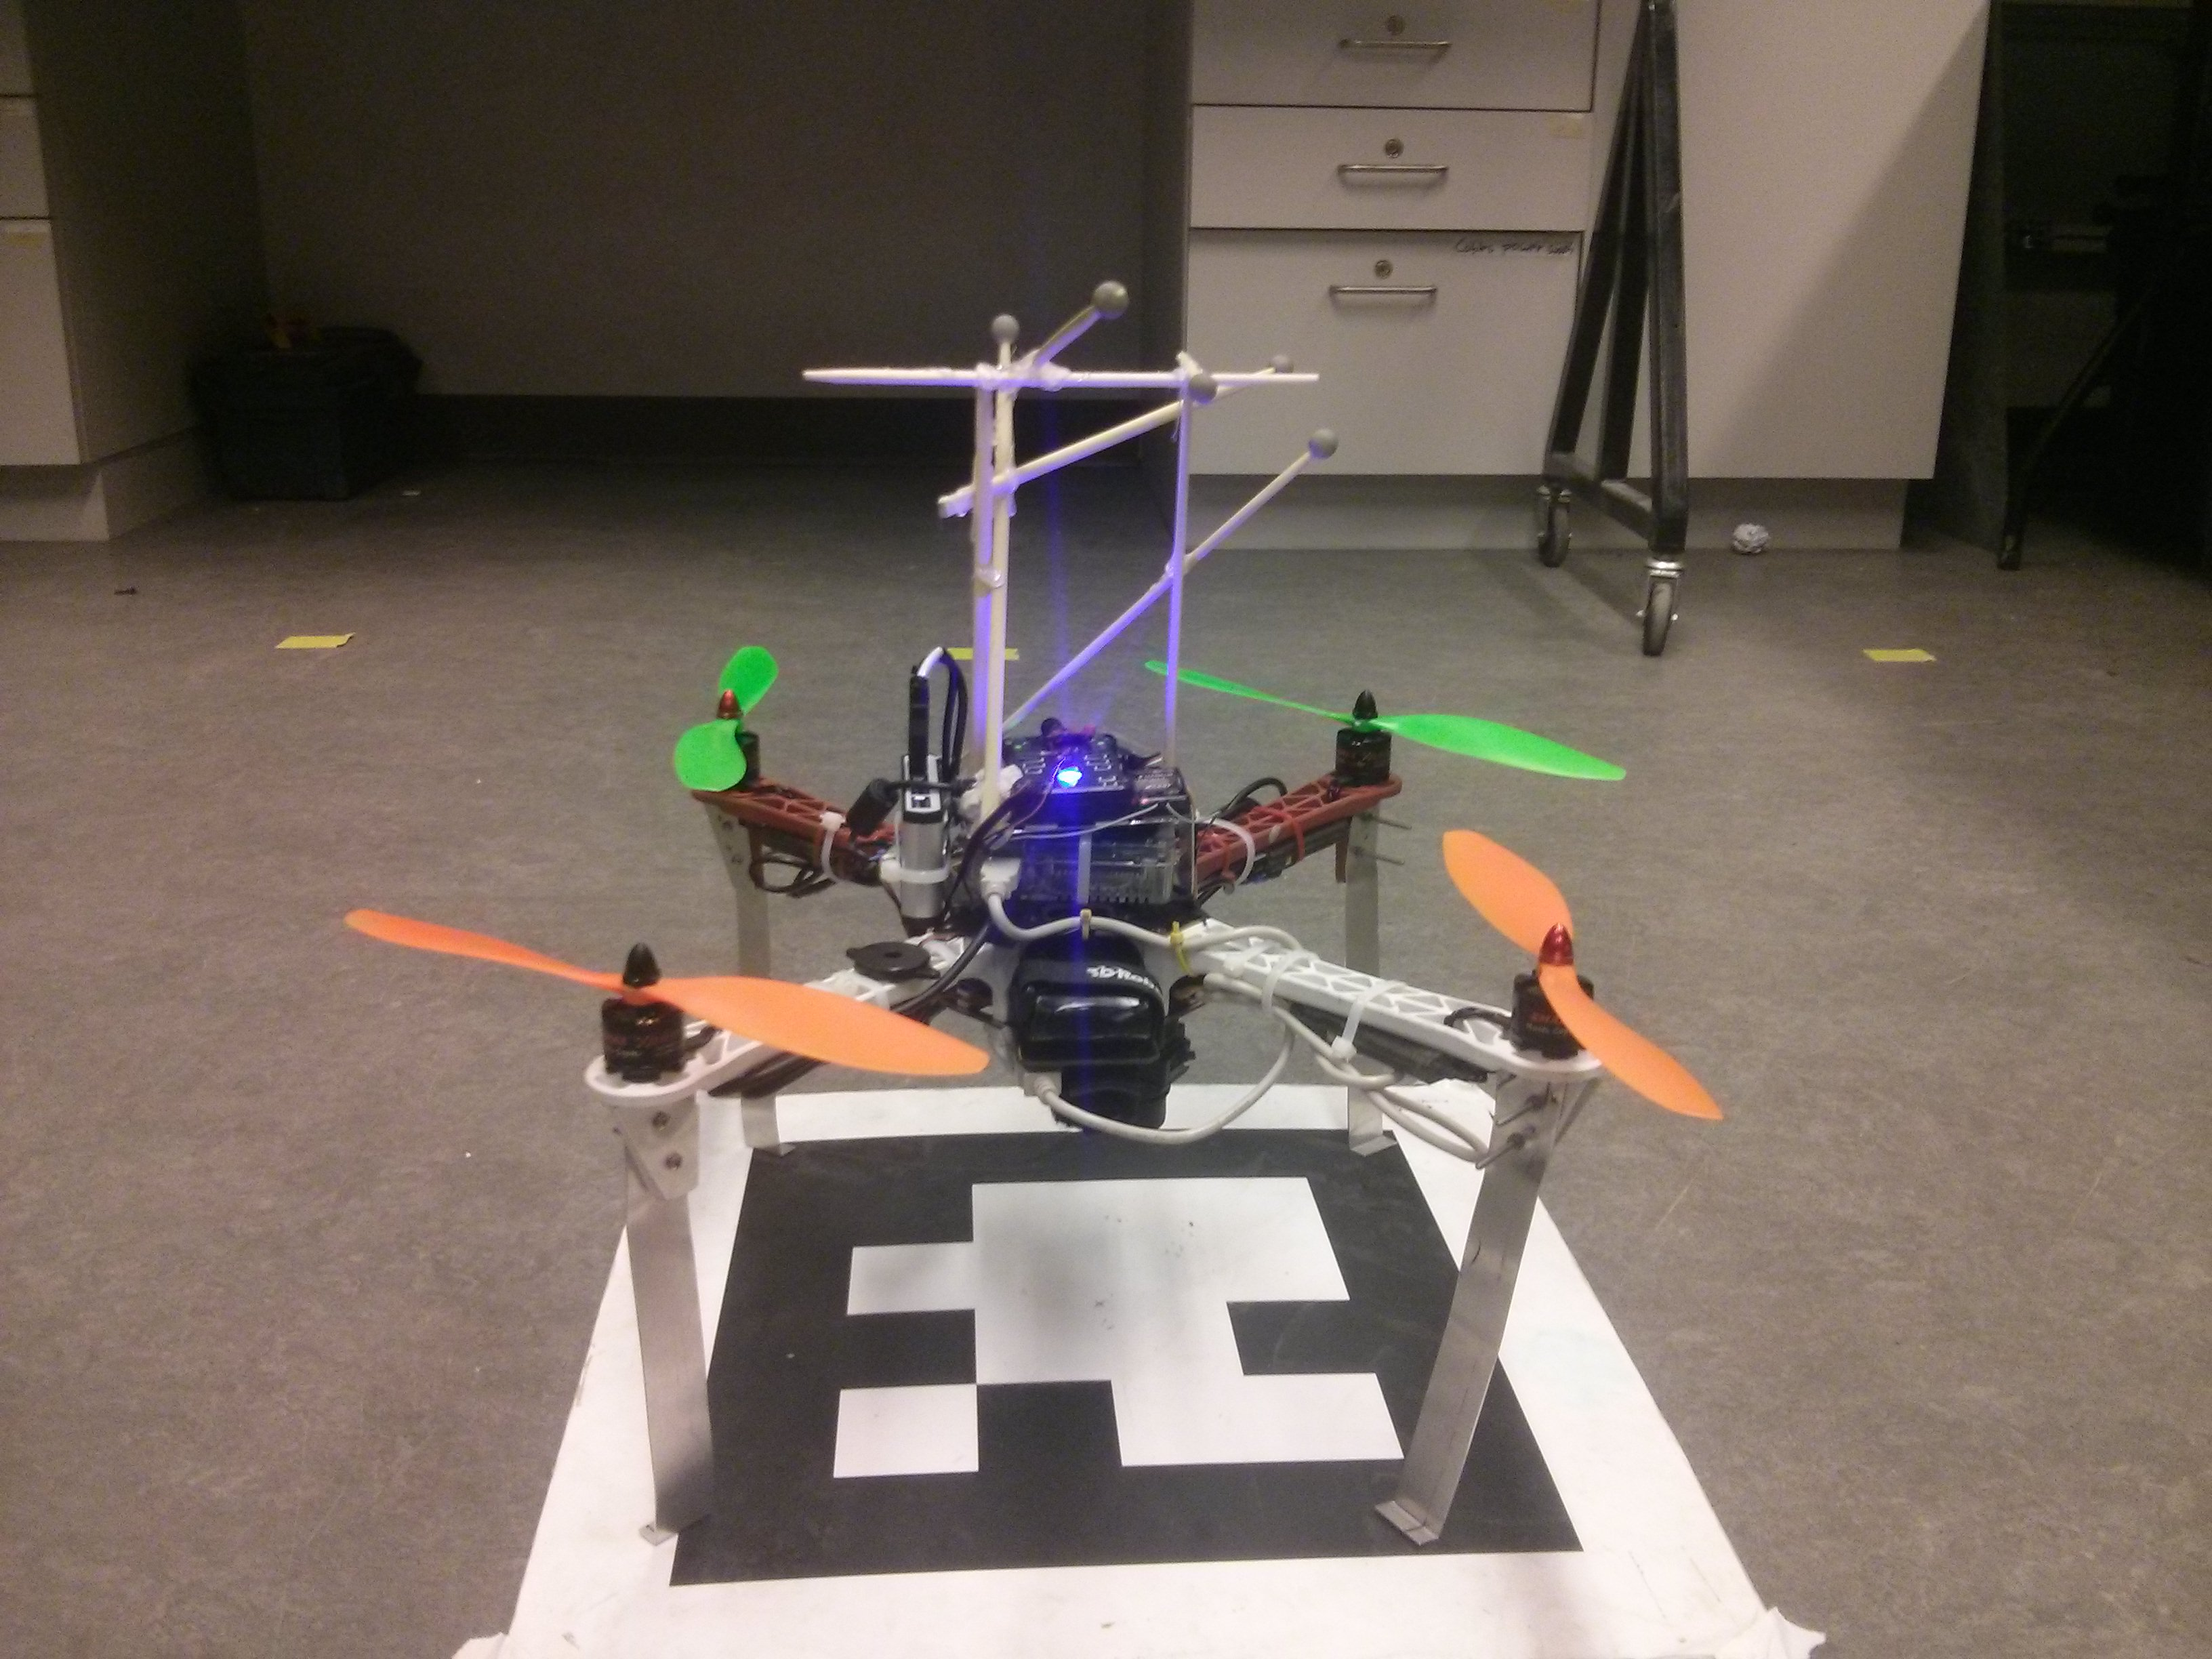
\includegraphics[width=\linewidth]{images/quad.jpg}
\end{frame}


\begin{frame}
    \frametitle{Pixhawk}
    \begin{center}
    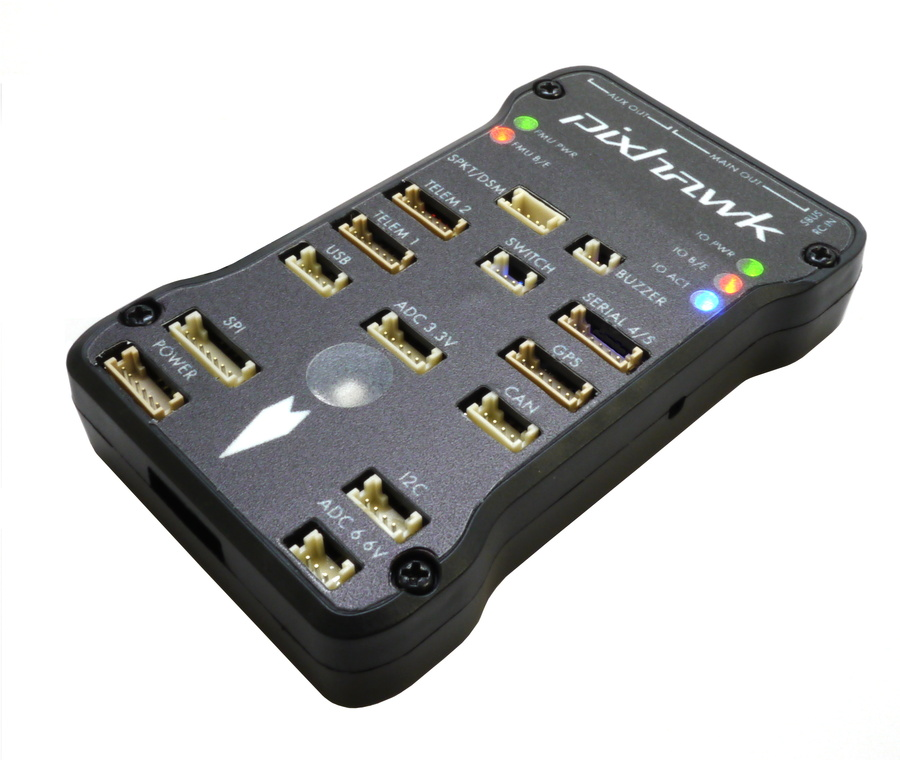
\includegraphics[width=0.25\linewidth]{images/pixhawk_crappy_thing.jpg}
    \end{center}
    
    
    All in one flight controller that controls all them motors and maintains stability.
    	\begin{itemize}
        		\item Produced by 3DR robotics at a cost of 200 USD
        		\item Runs the PX4 and APM flight stacks (both open source)
        		\item Direct communication to the odroid via a package called mavros
        	\end{itemize}    
\end{frame}

\begin{frame}
	\frametitle{Progress throughout the term}
	Needless to say out goal for a term project was... \textit{ambitious}. Issues include:
	\begin{itemize}
        		\item Difficulties getting the Odroid to talk to the Pixhawk
        		\item Issues with finding and understanding the PX4 and mavros documentation 
        		\item Several parameters in QGroundcontrol that had to be set to make the quad work as expected
    \end{itemize}  
    
    \textbf{But enough with the whining...}

\end{frame}

\begin{frame}
	\frametitle{Solving the Pose Estimation Problem}
	We used the MIT AprilTags Library for pose estimation:
	\begin{itemize}
	\item Uses a special type of 2D marker
	\item Processing entire images resulted in very slow pose estimates (3 - 5 Hz) on the Odroid. Down sampling increased frame rate but reduced the range to 1.5 meters.	
	\item  Varied down sampling size dynamically depending on the distance between the quad and the AprilTag
	\item AprilTag Inception (Tag within a tag to solve FOV problems)
	\item Black out image other than ROI
\end{itemize}

\end{frame}


\begin{frame}
	\frametitle{Proposed Method to solve the landing problem}
	 Our proposed method breaks down the landing problem into three separate parts:
	\begin{enumerate}
	\item \textbf{Detect} April Tag and get initial pose
	\item \textbf{Align} the font of the quad with the current location of the landing zone.
	\item \textbf{Move} towards the landing zone by pitching towards the landing zone
	\item \textbf{Descend} once the quad is located over the landing zone with PID controller
	\end{enumerate}
	
	We call this the \textbf{DAMD} approach
	
\end{frame}
\begin{frame}
\title{Testing out method}
The WAVELab has a motion capture system (MOCAP) that we used to test our code that we ran on the Odroid. Some of the results are shown in the following videos that show the quad moving tracing a square and then from last night, landing on the AprilTags \\

\href{https://www.youtube.com/watch?v=9oUxANr1j0o}{Partial Success} \\
and of course a few fails along the way \\
\href{https://youtu.be/2i0S6vrP9oc?t=53}{fails}

\end{frame}	

\begin{frame}
And here are some of the not so great moments we have had
\begin{itemize}
\item Early attempts at getting the quad to just take off: 
	\begin{itemize}
		\item \hyperlink{https://youtu.be/a6_0YQt9BuM?t=29}{\beamergotobutton{test}} \\
		\item \hyperlink{https://youtu.be/9zpM9thEneg?t=10}{\beamergotobutton{}} \\
		\item \hyperlink{https://youtu.be/5U7R6-7MHrY?t=137}{\beamergotobutton{}}
	\end{itemize}
\item MOCAP dropping out and causing the quad to crash:
		\item \hyperlink{https://youtu.be/ZHCqoEdYbX0?t=30}{\beamergotobutton{crash}}

\item And here is how we tested to see if our commands made sense:
\href{https://youtu.be/0EvrlYkYMyY?t=175}{command checking}

\end{itemize}

\end{frame}

\begin{frame}
\frametitle{Conclusion}
We have put a lot of hours into the project but greatly underestimated the time required to actually implement even the simple ideas that we came up for this project. \\

\textit{However} we did get the quad to land (sort of). And so...
\end{frame}

  \begin{frame}
    \frametitle{In summary..}
    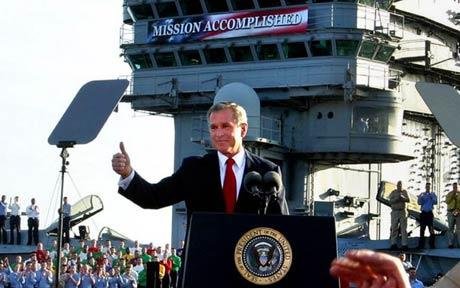
\includegraphics[width=\linewidth]{images/mission_accomplished.jpg}
\end{frame}

% etc
\end{document}